GoのソースコードにはPlan 9 CとAT\&Tコンパイラを使って書かれている部分があります。もしソースコードからインストールしたい場合は、あらかじめCのコンパイルツールをインストールしておく必要があります。

Macでは、Xcodeに適切なコンパイラが含まれています。

Unixでは、gccなどのツールをインストールする必要があります。例えばUbuntuではターミナルで\texttt{sudo apt-get install gcc libc6-dev}を実行することでコンパイラをインストールすることができます。

Windowsでは、MinGWをインストールする必要があります。その後MinGWでgccをインストールして、適切な環境変数を設定します。

直接オフィシャルサイトからソースコードをダウンロードできます。対応する\texttt{goVERSION.src.tar.gz}のファイルをダウンロードし、\texttt{\$HOME}ディレクトリに解凍してから以下のコマンドを実行します。

\begin{lstlisting}[numbers=none]
cd go/src
./all.bash
\end{lstlisting}

all.bashを実行後"ALL TESTS PASSED"が表示されると、インストール成功です。

上記はUnixスタイルのコマンドです、Windowsもインストール方法は似ており、\texttt{all.bat}を実行するだけです。コンパイラはMinGWのgccを使います。

もしMacまたはUnixユーザであればいくつかの環境変数を設定する必要があります。再起動しても有効にしたい場合は以下のコマンドを\texttt{.bashrc}や\texttt{.zsh}に書いておきます。

\begin{lstlisting}[numbers=none]
export GOPATH=$HOME/gopath
export PATH=$PATH:$HOME/go/bin:$GOPATH/bin
\end{lstlisting}

ファイルに書き込んだ場合は、\texttt{bash .bashrc}や\texttt{bash .zshrc}を実行してすぐに設定を有効にします。

Windowsシステムの場合は、環境変数を設定する必要があります。pathにgoが存在するディレクトリを追加し、gopath変数を設定します。

設定が終わり、コマンドプロンプトで\texttt{go}を入力すると、下図のような画面が表示されるはずです。

\begin{figure}[H]
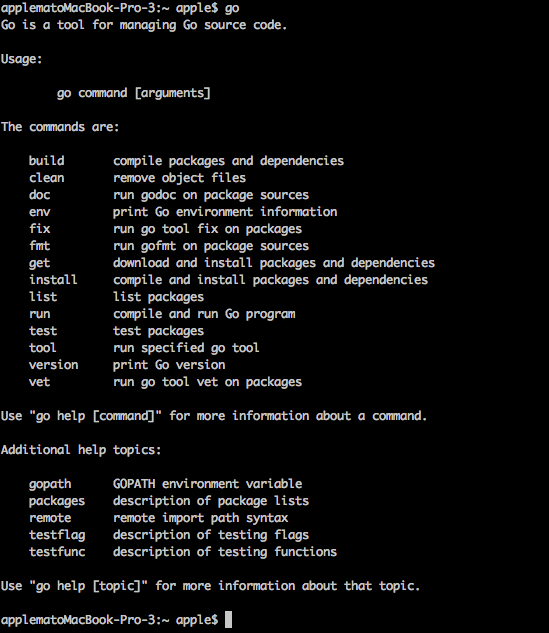
\includegraphics[width=14cm]{1.1.mac.png}
\label{図1.1}
\caption{ソースコードインストール後Goコマンドを実行}
\end{figure}

GoのUsage情報が表示されれば、Goのインストールは成功です:もしこのコマンドが存在しない場合は、PATH環境変数のなかにGoのインストールディレクトリが含まれているか確認してください。

\begin{quote}
  GOPATHについては以降の章で詳しくご説明します
\end{quote}



